% Geometry setup
\documentclass[14pt,a4paper]{article}
\usepackage[margin=3cm]{geometry}

% Language setup
\usepackage[magyar]{babel} % Babel for Hungarian
\usepackage[T1]{fontenc} % Output character encoding
\usepackage[utf8]{inputenc} % Input character encoding

% Spacing setup
\setlength{\parindent}{0pt} % No paragraph indenting
\setlength{\parskip}{5pt} % Set spacing between paragraphs
\frenchspacing
\newcommand{\rmspace}{\vspace{-19pt}}

% Dependency setup
\usepackage{amsmath}
\usepackage{amssymb}
\usepackage{listings}
\usepackage{float}
\usepackage{graphicx}
\usepackage{hyperref}
\usepackage{url}
\usepackage[comma,authoryear]{natbib}

% Python pretty print
\usepackage{minted}
% End Python setup

% Hyperlink format
\usepackage{xcolor}
\hypersetup{
    colorlinks,
    linkcolor={red!50!black},
    citecolor={blue!50!black},
    urlcolor={blue!80!black}
}
% End Hyperlink format

% Title setup
\title{Nagyadat Coolmini}
\author{Gesztesy Tamás, Nemkin Viktória}
\date{}

% Document
\begin{document}
\maketitle

\section{Bevezetés}

Az elkészült programkódok és az adathalmazok elérhetőek a
\href{https://www.github.com/nemkin/cool-mini-or-not}{\url{https://www.github.com/nemkin/cool-mini-or-not}} webcímen.

\section{Feladat}

A félév során a Cool Mini Or Not weboldal (\href{http://www.coolminiornot.com}{\url{http://www.coolminiornot.com}})
adatelemzésével foglalkoztunk.

Az Cool Mini Or Not weboldal egy figurafestésekre specializálódott közösségi oldal, ahova a kifestett miniket
lehet feltölteni, a többi felhasználó pedig szavazhat és kommentelhet a fotóinkra.

\begin{figure}[H]
\centering
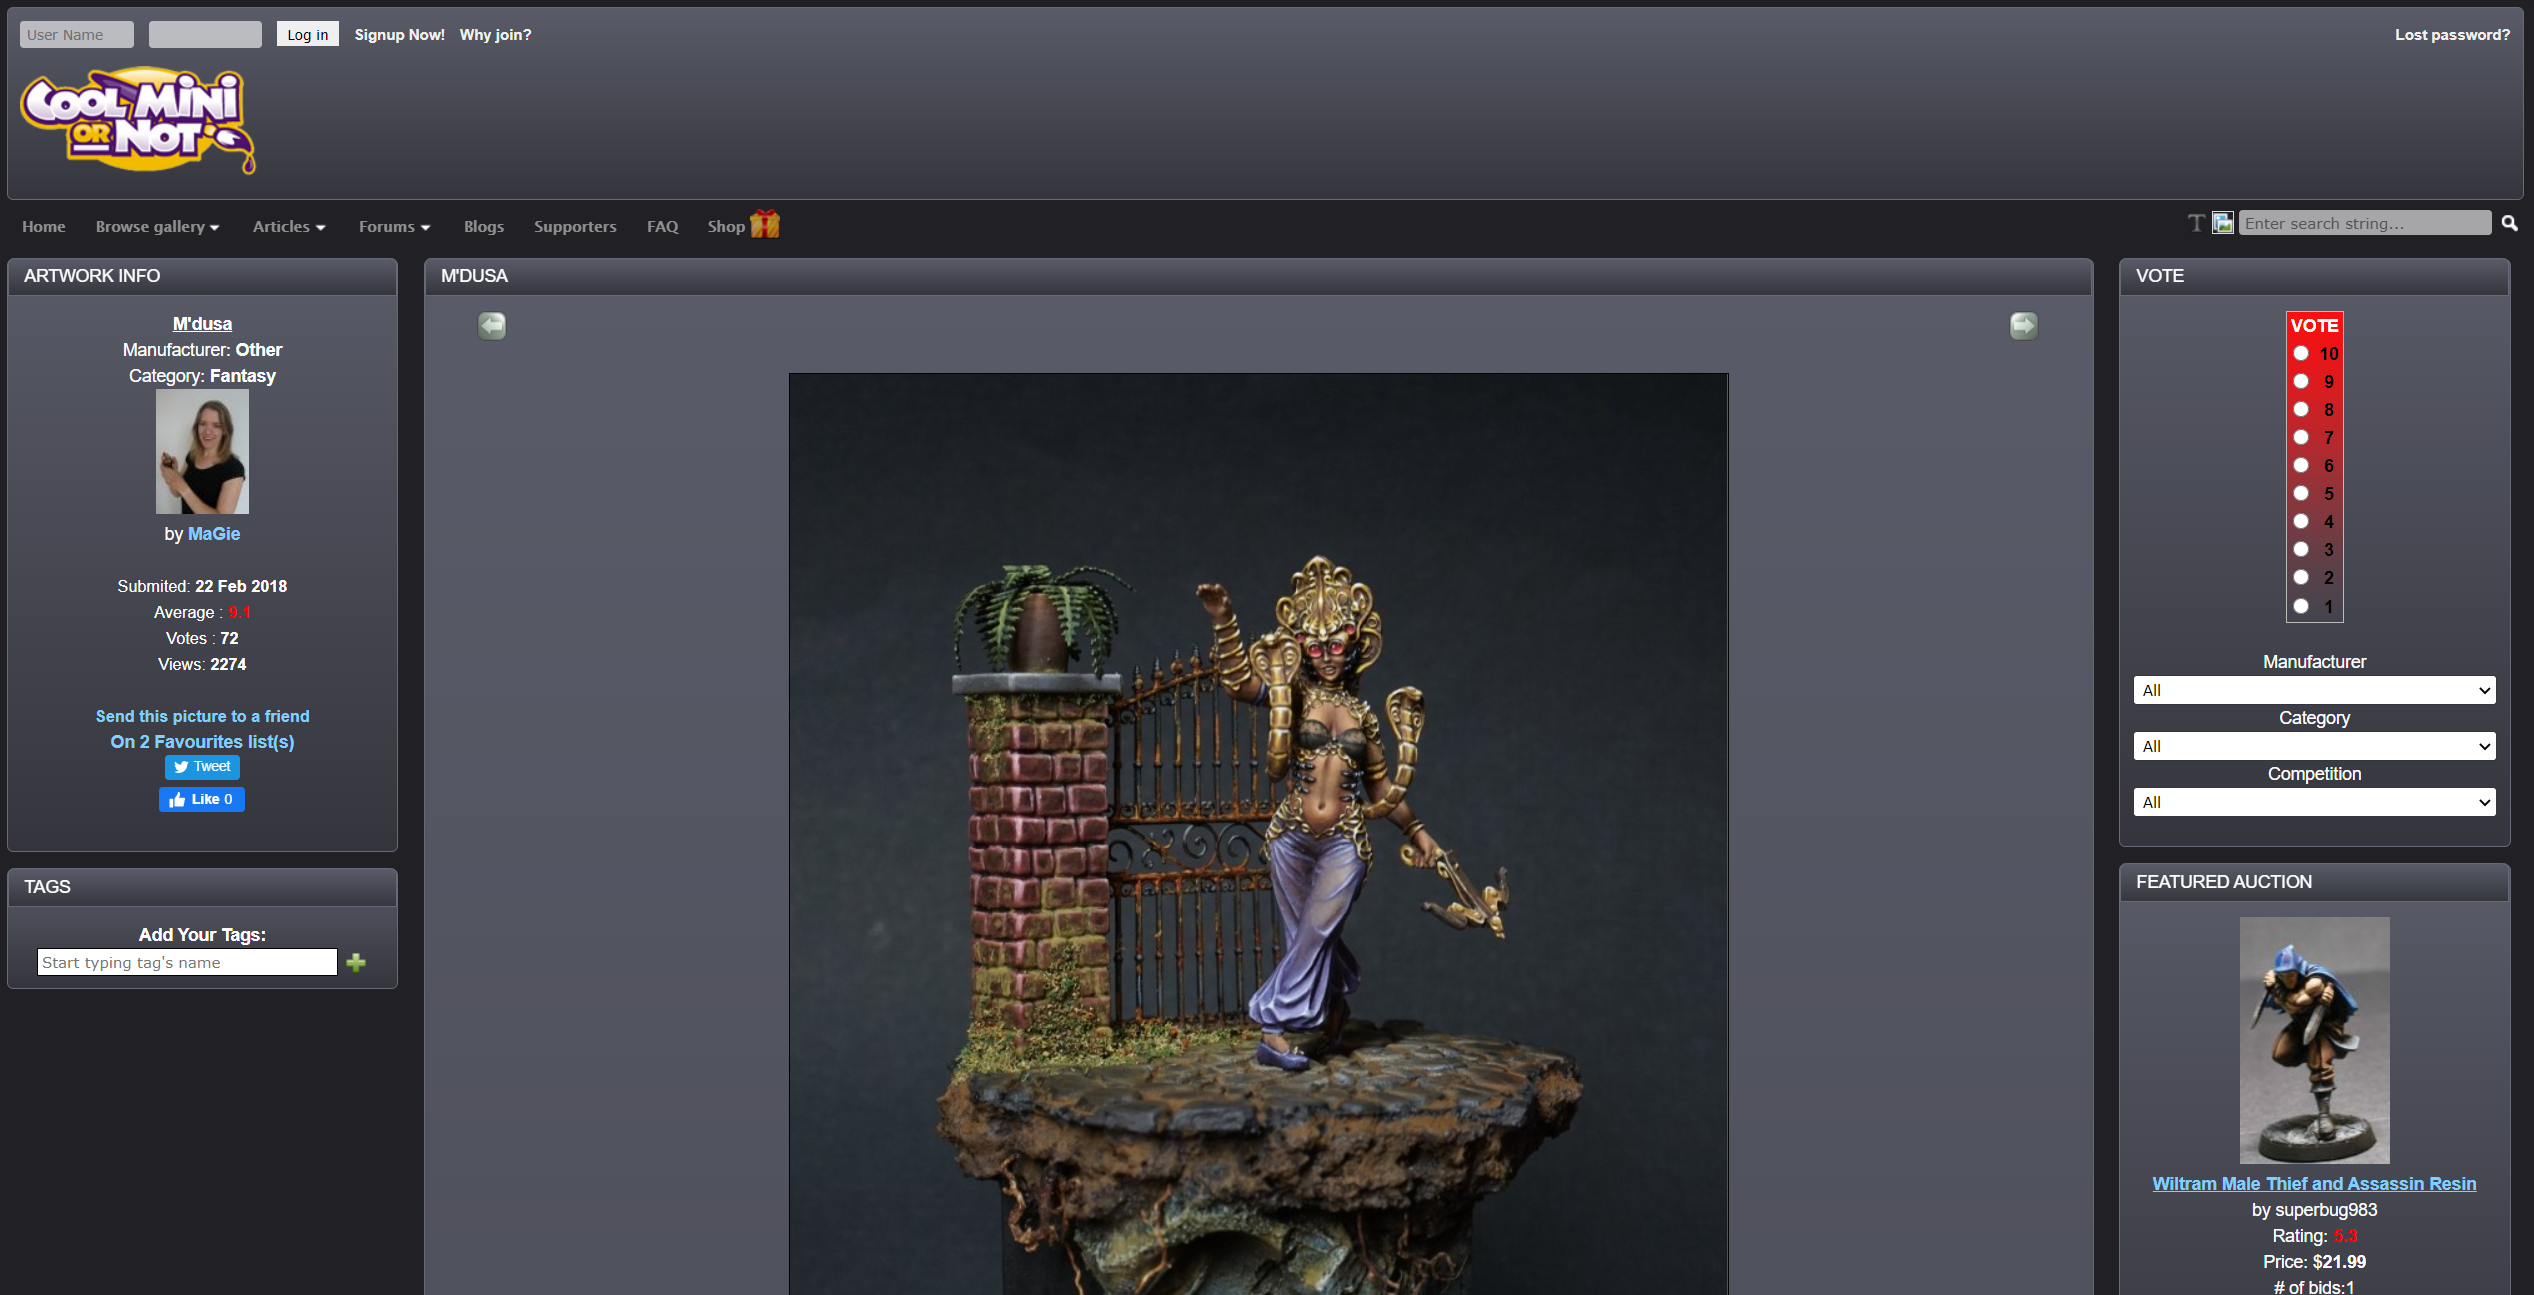
\includegraphics[width=1.0\columnwidth]{pics/page_submission.png}
\caption{Coolmini feltöltés}
\end{figure}

\begin{figure}[H]
\centering
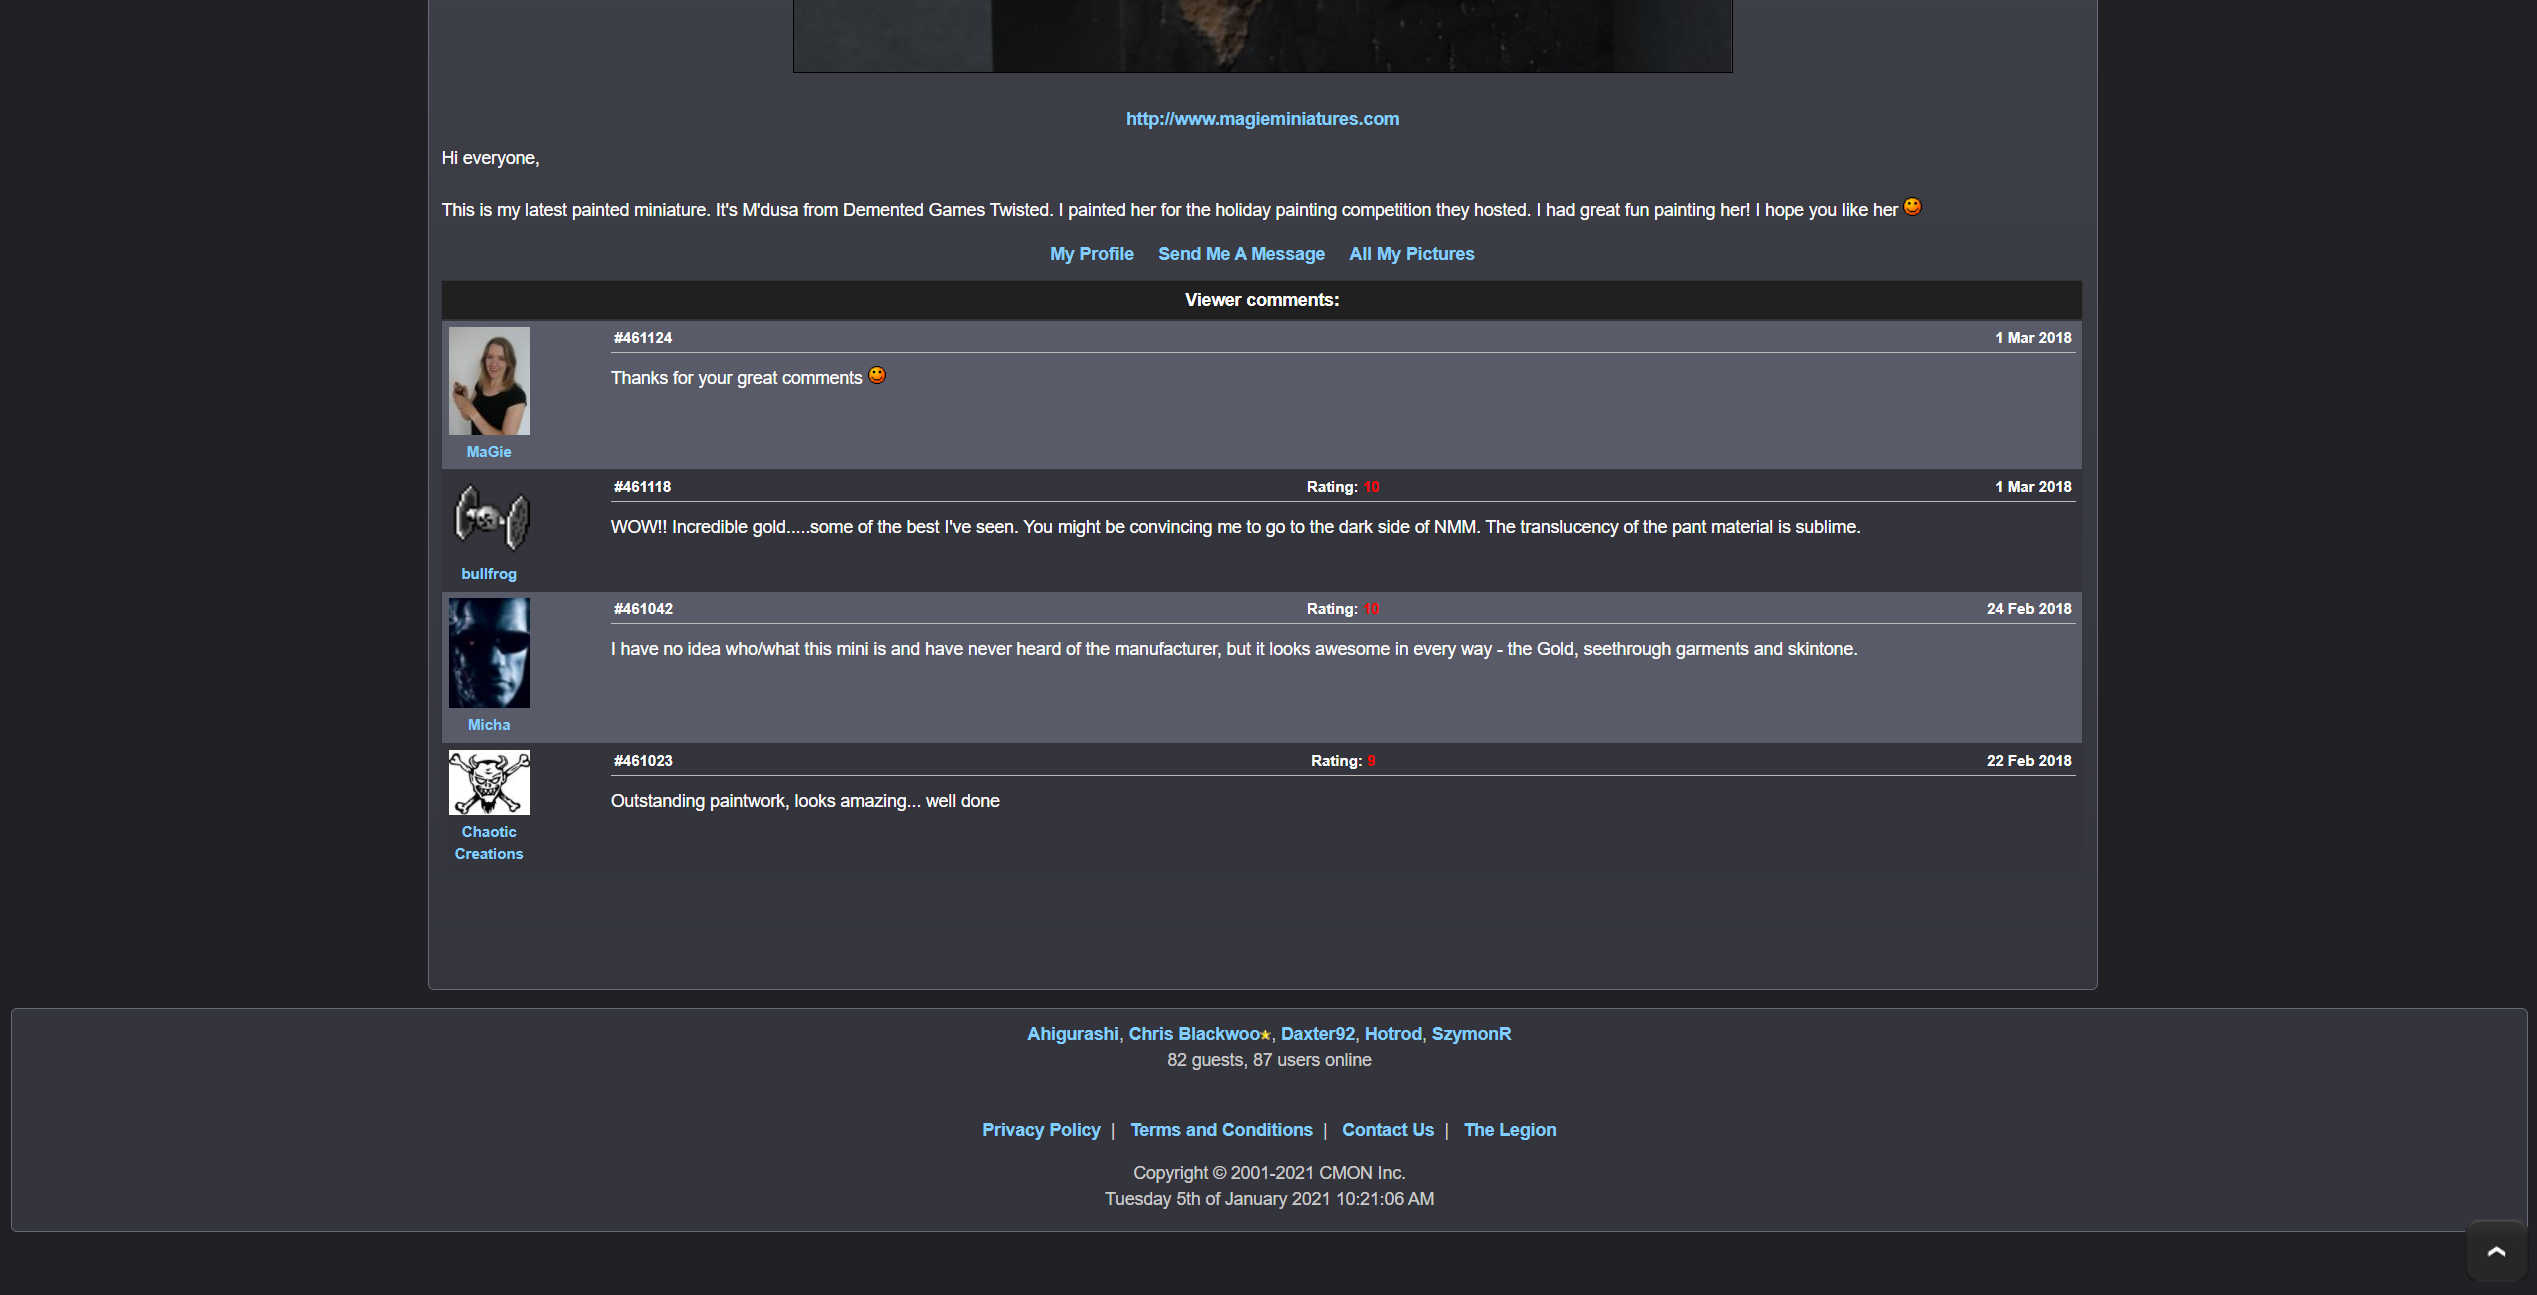
\includegraphics[width=1.0\columnwidth]{pics/page_comments.png}
\caption{Coolmini feltöltés}
\end{figure}

\section{Adathalmaz letöltése}

Az első feladat a weboldal adatainak a kinyerése volt. Ez általában egy nehézkes és körülményes feladat. Nagy
méretű adathalmazról van szó, több 10 GB-nyi adat, melyet napokon keresztül tudunk csak letölteni. Általában a
weboldalak üzemeltetői nem szeretik az ilyen jellegű letöltéseket, ezért előfordulhat, hogy blokkolják az IP
címünket (például DDOS támadásnak hiszik a letöltést).

Szerencsére azonban a weboldal tartalma archiválva lett a Wayback Machine által
(\href{https://web.archive.org/web/2020*/coolminiornot.com}{\url{https://web.archive.org/web/2020*/coolminiornot.com}}),
ehhez pedig már létezik letöltő script
(\href{https://github.com/hartator/wayback-machine-downloader}{\url{https://github.com/hartator/wayback-machine-downloader}}).

A letöltő scriptet Raspberry Pi-n keresztül futtattam, mivel összesen 2 héten keresztül tartott a letöltés.

Sajnos problémát jelentett, hogy bizonyos régebbi bejegyzések rossz formátumban töltődtek le az oldalról, ezért egyéb
letöltési lehetőségekkel is próbálkoztam (wget), azonban ezekben az esetekben a felhasználók kommentjeit nem lehetett
letölteni, ezért végül az eredeti adathalmazt használtam fel, a hibás fájlok kiszűrésével.

\section{Transzformáció}

A következő feladat az adatok kinyerése volt a HTML fájlokból. Ehhez az LXML nevű Python modult használtam, melynek
segítségével XML fájlokat lehet parsolni. A következő python program segítségével készítettem el az adathalmazt:

\inputminted[linenos, breaklines, fontsize=\footnotesize]{python}{../python/process.py}

A következő csv fájlokat hoztam létre:

\paragraph{Submissions}

A submissions fájl tartalmazza soronként 1-1 feltöltött mini adatait:

\begin{itemize}
\item entry\_id
\item entry\_date
\item entry\_name
\item entry\_image: A képhez tartozó url cím.
\item user\_id
\item user\_name
\item manufacturer
\item category
\item view\_count
\item vote\_count
\item vote\_average
\end{itemize}

\begin{figure}[H]
\centering
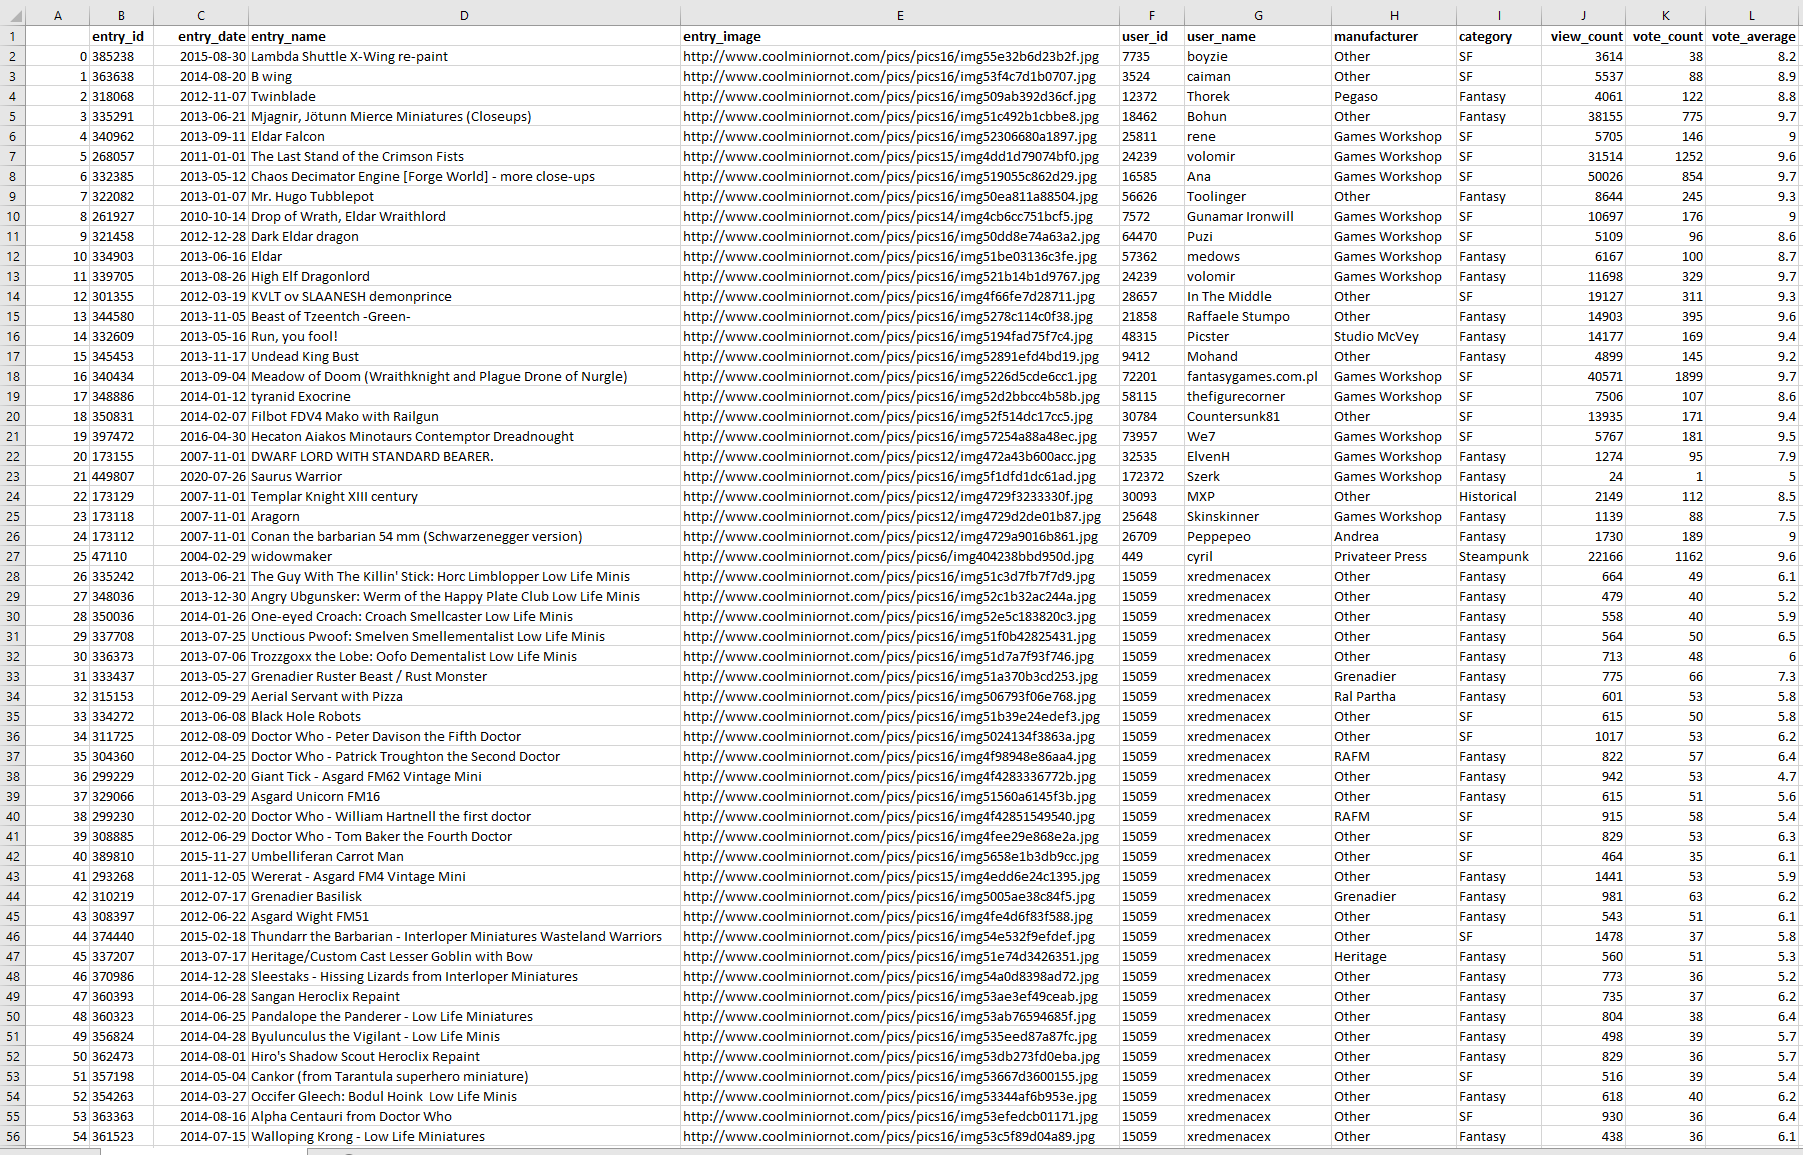
\includegraphics[width=1.0\columnwidth]{pics/csv_submissions.png}
\caption{submissions.csv}
\end{figure}

\paragraph{Comments}

A comments fájl tartalmazza soronként a minikhez adott kommenteket. Az entry\_id-val azonosítom, hogy a komment
melyik feltöltéshez érkezett:

\begin{itemize}
\item entry\_id
\item comment\_id
\item comment\_date
\item commenter\_user\_id
\item commenter\_user\_name
\item vote
\item comment
\end{itemize}

\begin{figure}[H]
\centering
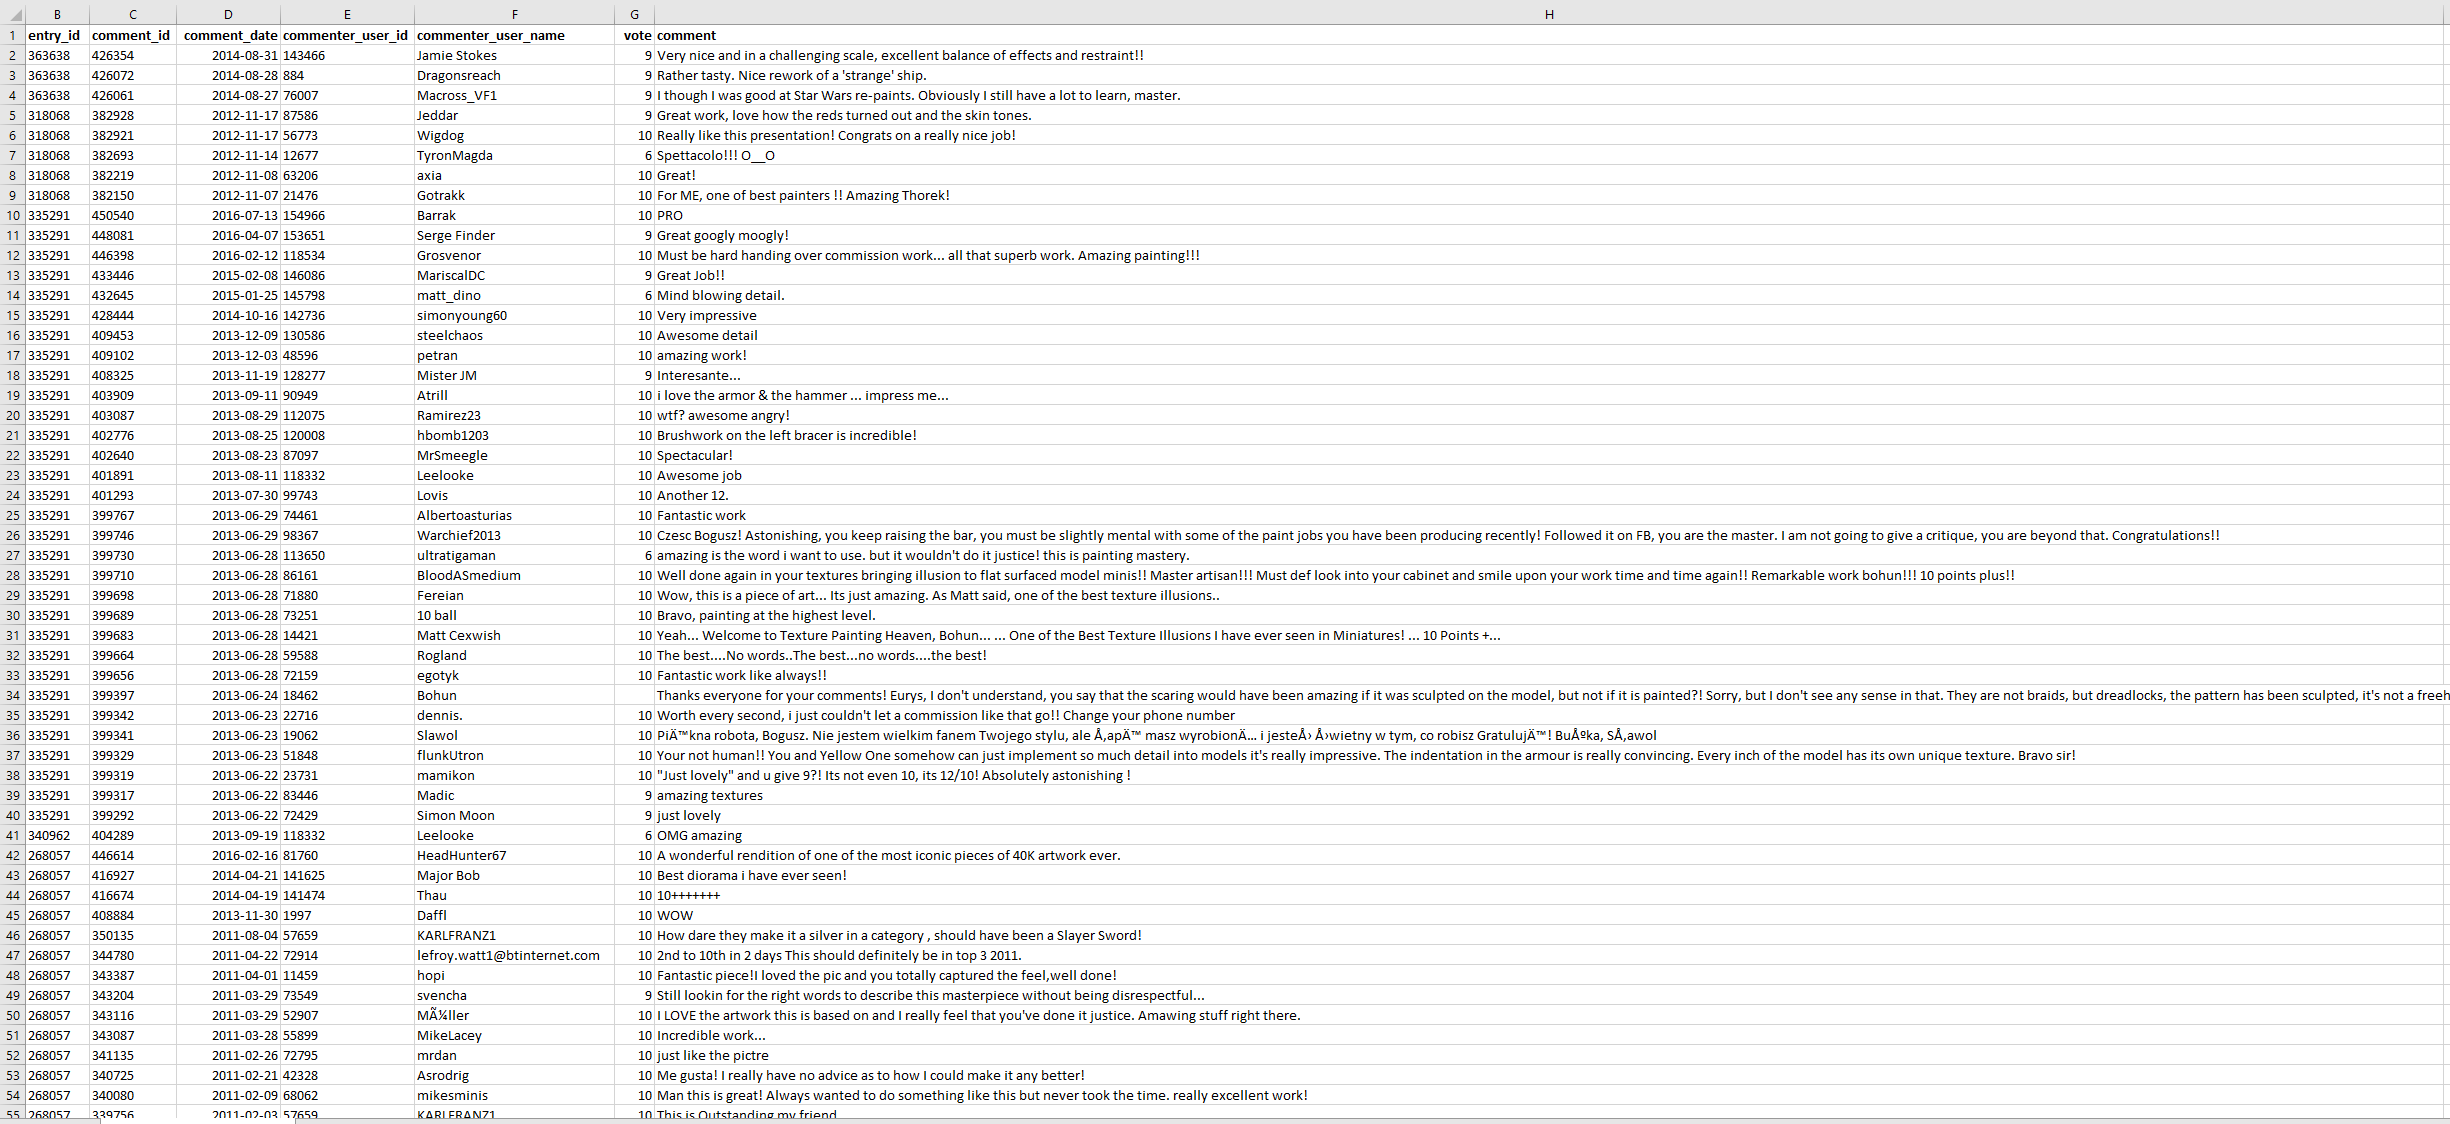
\includegraphics[width=1.0\columnwidth]{pics/csv_comments.png}
\caption{comments.csv}
\end{figure}

\paragraph{Ebay}

A feltöltött minik egy részéhez tartozik ebay link, ahol licitálni lehet azok megvásárlására. Ezt egy külön
adathalmazban rögzítettem.

\begin{itemize}
\item entry\_id
\item ebay\_id
\item ebay\_current\_price
\item ebay\_first\_bid
\item ebay\_number\_of\_bids
\item ebay\_end\_date
\end{itemize}

\begin{figure}[H]
\centering
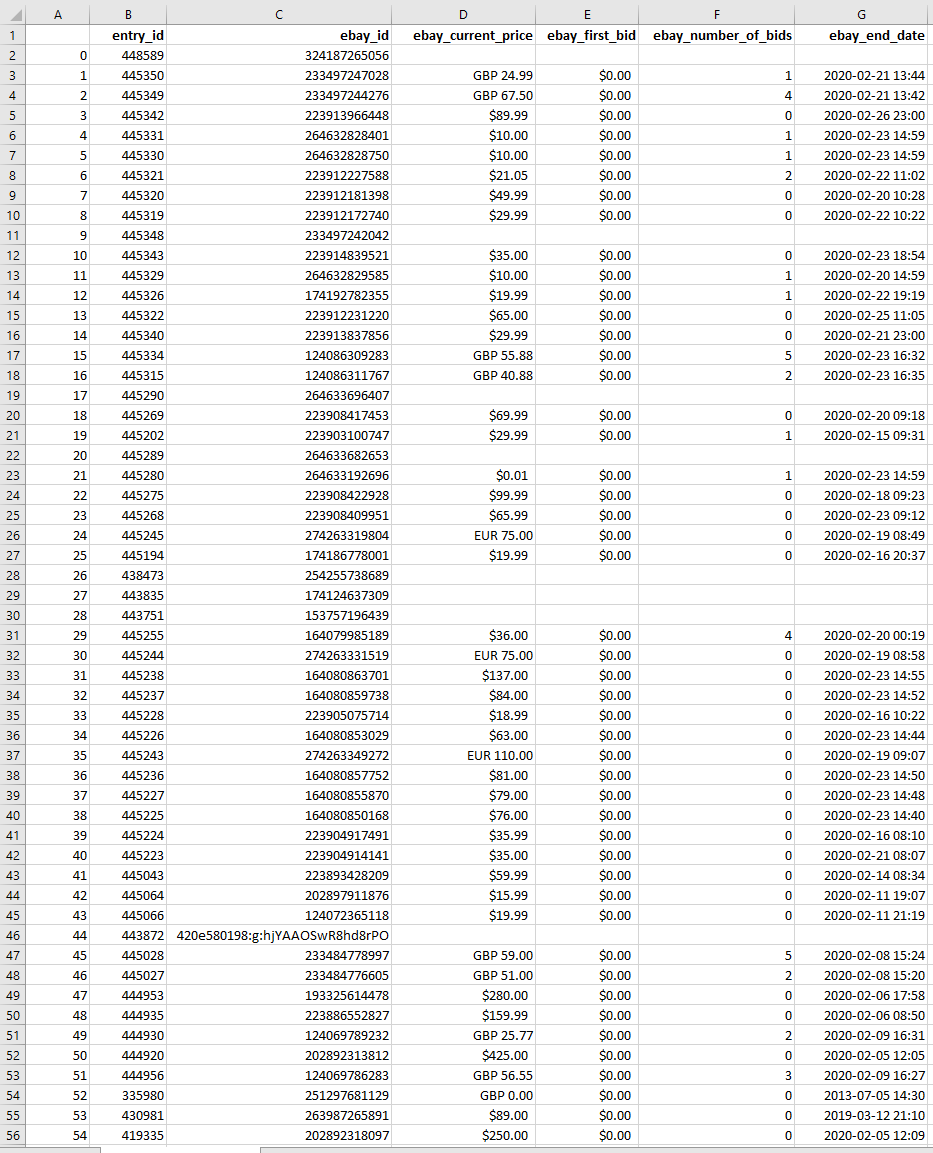
\includegraphics[width=1.0\columnwidth]{pics/csv_ebay.png}
\caption{ebay.csv}
\end{figure}

\section{Online ajánlórendszer}

Az ajánlórendszer Item-based Collaborative Filtering alapon működik az ajánlórendszerek házihoz megosztott
Recommender Systems, \cite{sammut_encyclopedia_2010} könyvből vett fejezet és az ott hivatkozott
\cite{linden_smith_york_2003} cikk alapján.

Ennek célja, hogy online, real-time képesek legyünk miniket ajánlani egy felhasználónak, miközben a miniket értékeli.
A felhasználók összehasonlításán alapuló rendszerek esetében az aktív felhasználó korrelációit minden szavazat után
újra kellene számolni, ami online módon nagyon erőforrásigényes lenne. Ezzel szemben, az item-alapú ajánlórendszert
használva előre ki tudtam számolni a minik közötti korrelációkat. Ezt egy nagy méretű json fájlban tároltam el,
mely
\href{https://raw.githubusercontent.com/nemkin/cool-mini-or-not/main/data/correlations.json}{ezen a linken}
tekinthető meg.

Látható, hogy sok mininek 1.0, illetve -1.0 a korrelációja, ez abból adódik, hogy egyetlen felhasználó
a kapcsolat közöttük, ez a felhasználó pedig ugyanazt a szavazatot adta mindkét minire.

Az ajánlórendszerhez készült egy egyszerű Angular-os weboldal, mely így néz ki:

\begin{figure}[H]
\centering
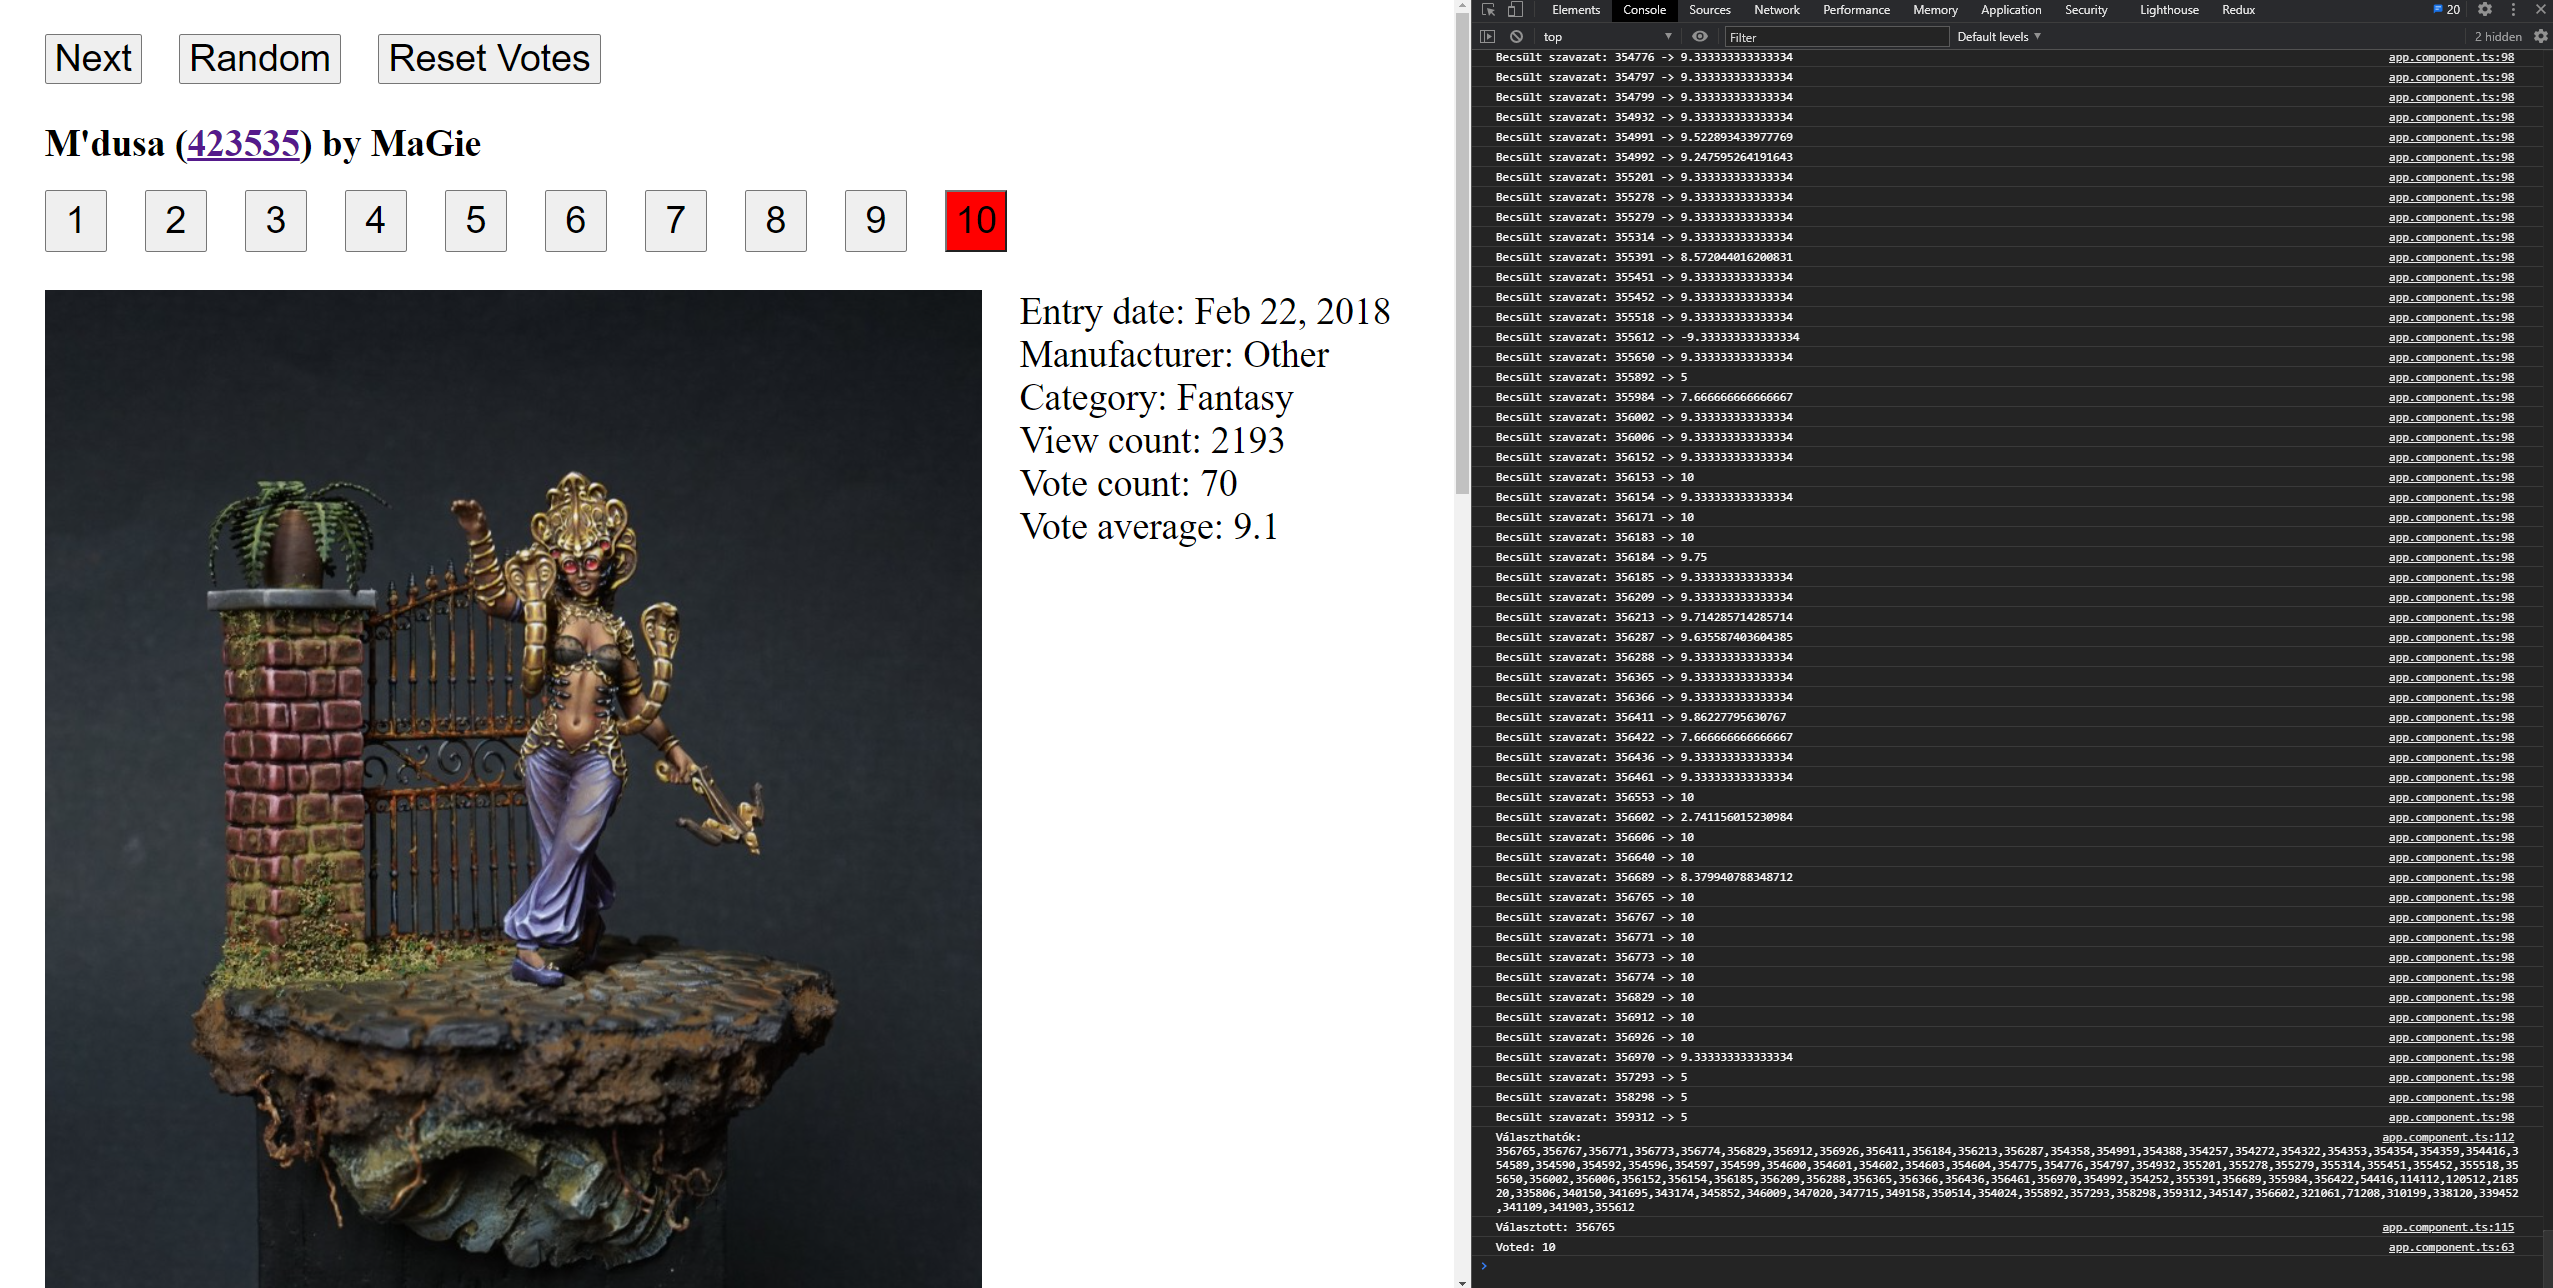
\includegraphics[width=1.0\columnwidth]{pics/ajanlorendszer.png}
\caption{Ajánlórendszer}
\end{figure}

A Next gombra kattintással lehet kérni a következő ajánlott minit, a Random gombra kattintással
véletlen minit kérhetünk (ajánlórendszer nélkül), a Reset Votes gomb pedig törli az összes leadott
szavazatunkat.

Amini neve melletti entry\_id-ra kattintva az eredeti weboldalra navigálva megtekinthető az eredeti
beküldés. A számolások részeredményeit a konzolban lehet nyomonkövetni.

\section{Tanulságok}

A félév során nagyon sokat tanultam a feladat elkészítése során.

A letöltés sokkal bonyolultabb lett mint amire számítottam: A letöltött weboldalak néha teljesen másképp néztek ki
mint az élesek, például a kommentszekciót a wget teljesen kihagyta. A törött linkek nagyon sok problémát jelentettek,
amiket nagyon körülményes volt kijavítani, van ahol nem is sikerült (valószínűleg elmozgatták azokat a képeket az éles
website-on). Az adathalmaz méretéből fakadóan meg kellett oldani, hogy 2 héten keresztül zavartalanul fusson a letöltő,
problémát okozott például egy kiment biztosíték, ami miatt előről kellett kezdeni a letöltést. Az adatok mérete
szerencsére körülbelül 100 GB volt, de más adathalmaz esetében ebből is lehetett volna probléma. Emellett szerencsére
nem tiltották le az IP címemet, még mindig elérem a weboldalt, pedig más weboldalak esetében ez is megtörténhetett volna.

Az adatelemzés közben próbáltam különféle összefüggéseket találni az adatokban, rajzoltam grafikonokat, szavak
darabszámát elemeztem, ezen kódok egy része a
\href{https://github.com/nemkin/cool-mini-or-not/blob/main/python/analysis.py}{\url{https://github.com/nemkin/cool-mini-or-not/blob/main/python/analysis.py}}
linken megtalálható. A problémát az jelentette, hogy nem igazán találtam érdekes összefüggést, amelynek mentén el
lehetett volna indulni. Nem találtam olyan attribútumot az adathalmazban ami jelentősen meghatározta volna
a szavazatok alakulását, ez várható is volt hiszen a festés minősége a fő döntő elem.

Ezért végül egy ajánlórendszer elkészítése mellett döntöttem a szavazatok és a képek alapján. Itt szerettem volna
valamilyen interaktív megoldást adni, ezért választottam az Item-based Collaborative Filtering módszert, mert azzal
előre kiszámolt korrelációk alapján lehetett ajánlatokat adni. A korrelációk kiszámolása több órát vett igénybe,
ezt szavazatonként biztosan nem lehetett volna megvárni.

A weboldal használata közben észrevettem, hogy ha jó szavazatot adok egy mininek, akkor előfordul, hogy ahhoz hasonló
méretű, kinézetű (más felhasználó által feltöltött) miniket kapok legközelebb, ezért összességében valamilyen
összefüggést sikerült kihasználni a collaborative filtering módszerével.

\bibliographystyle{plainnat}
\bibliography{citations}

\end{document}


